\chapter{\iftoggle{german}{Evaluierung}{Evaluation}}\label{ch:evaluation}

\section{Domain gaps - Qualitative}
Visualize domain gap between S2R:3D-FREE and real image(pix3d)

Visualize domain gap between other synthetic dataset like 3dfront, scenenet
tsne

\begin{figure}
    \centering
    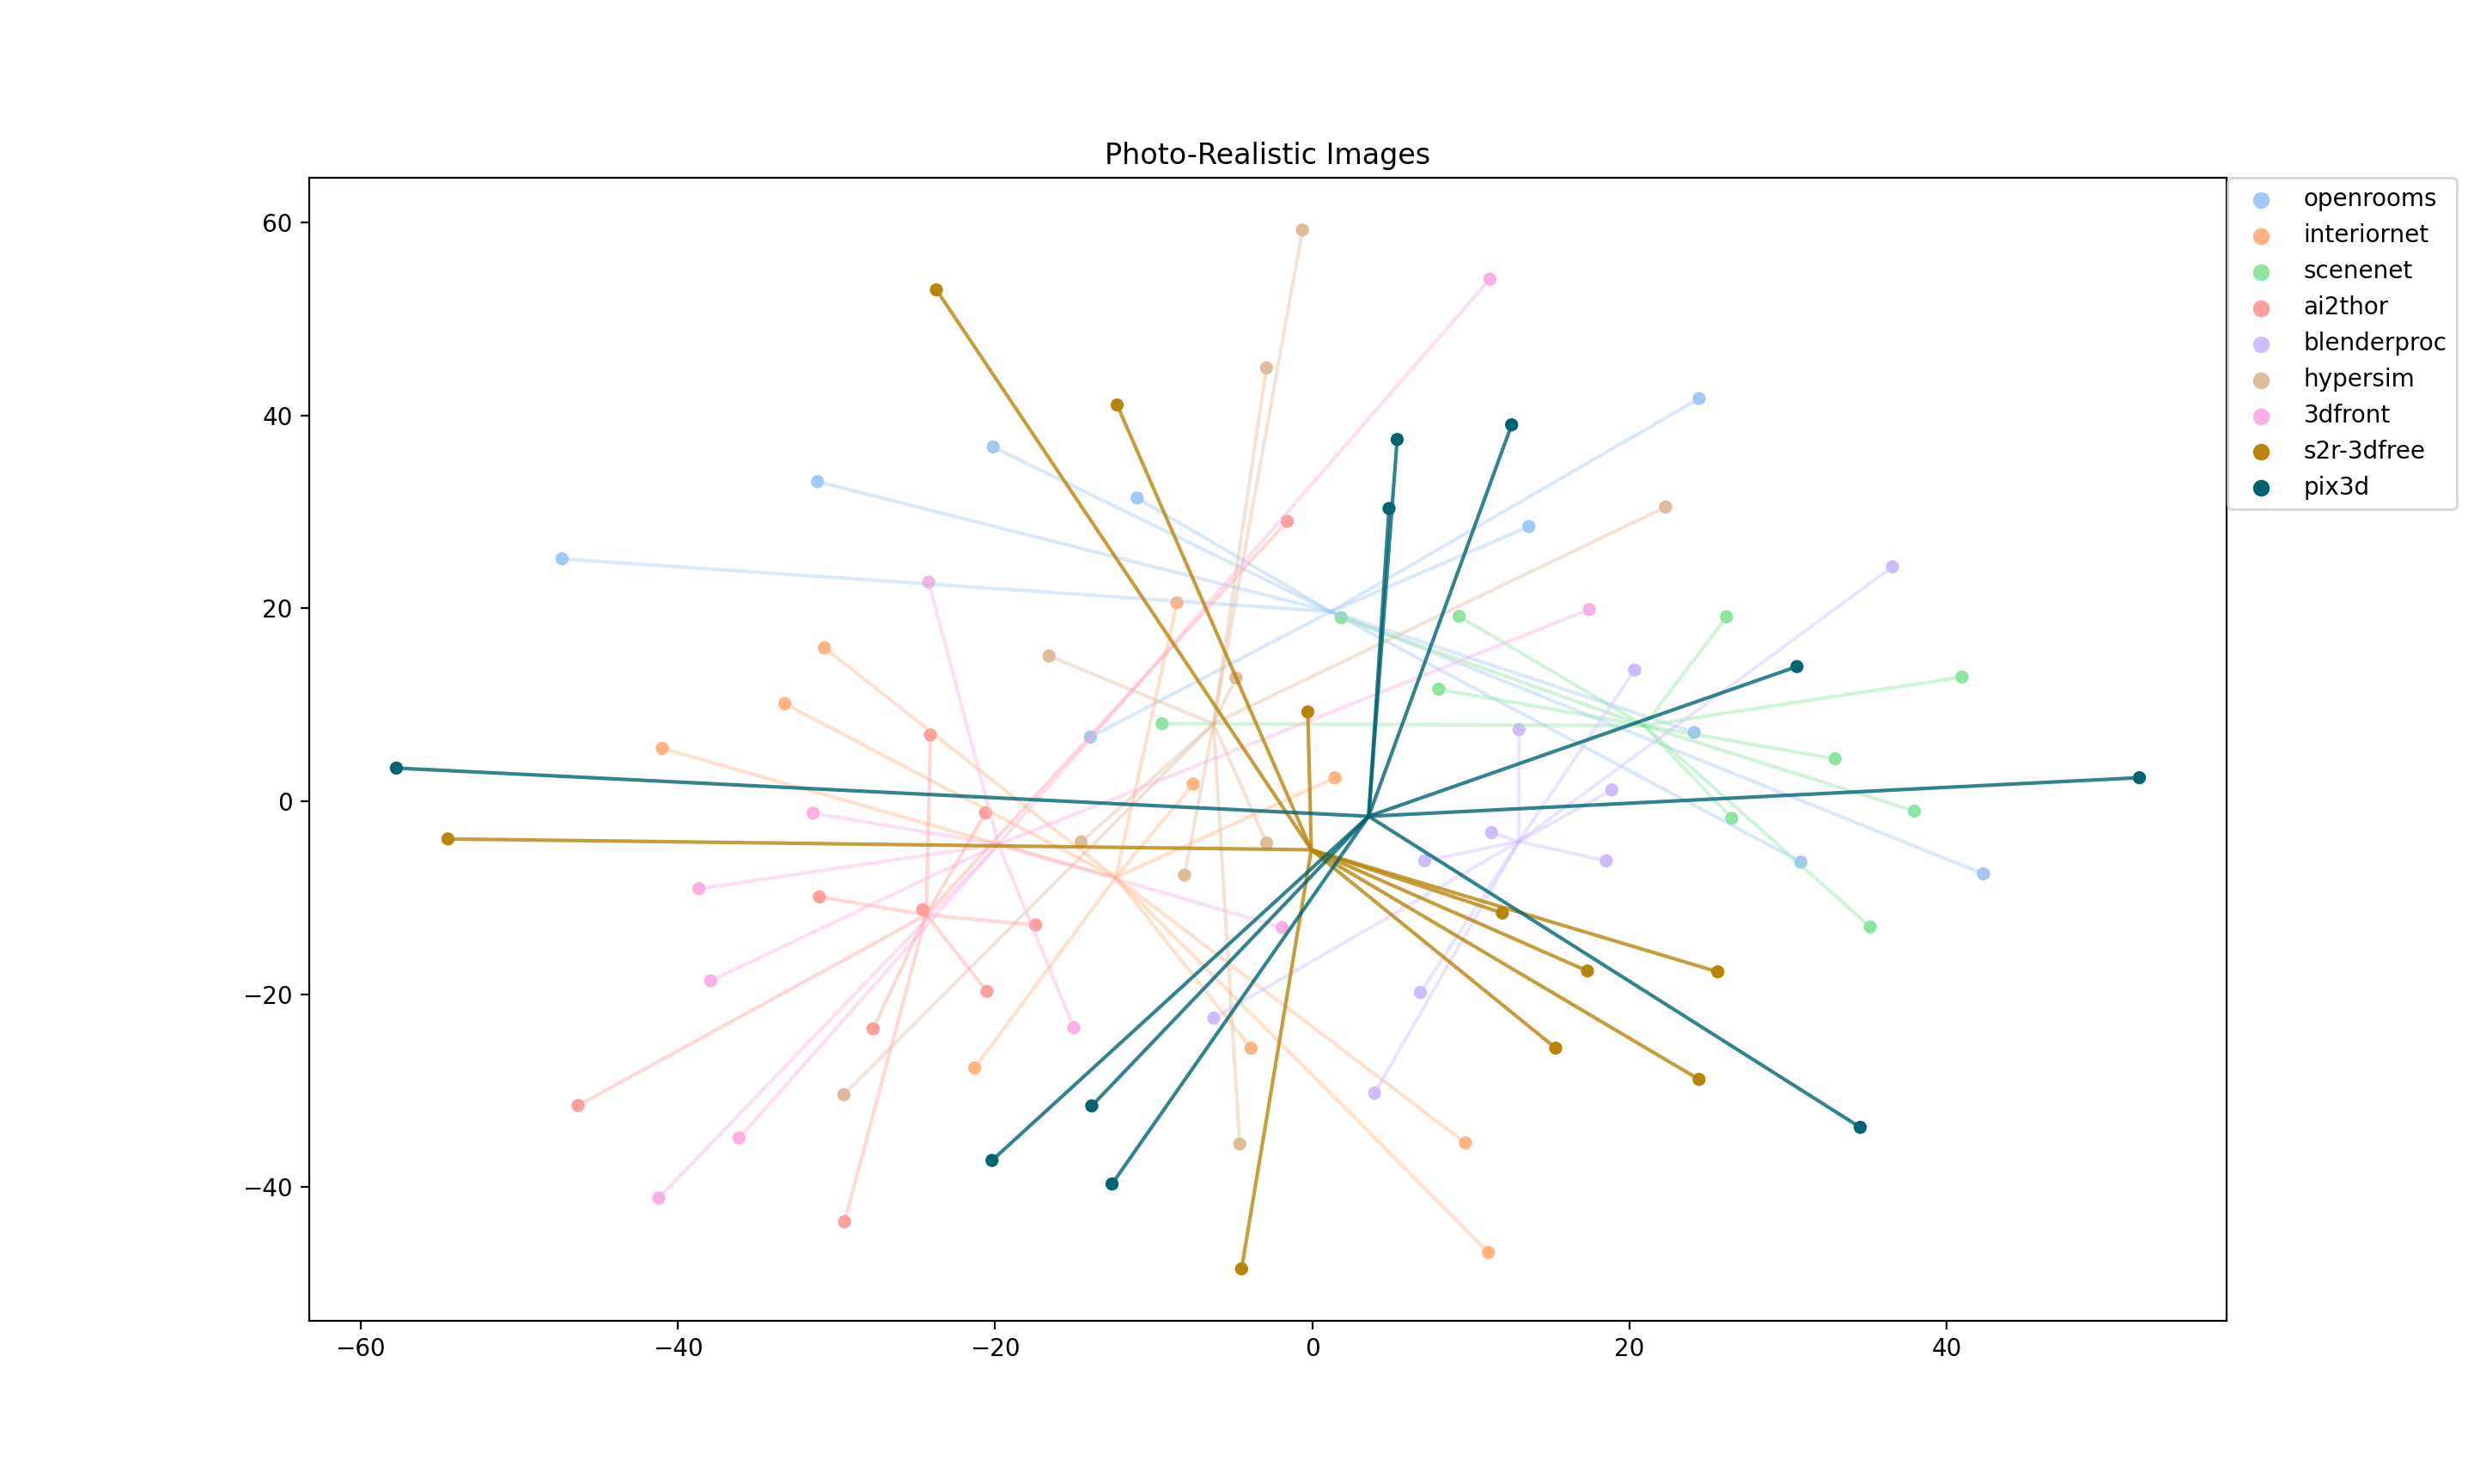
\includegraphics[width=\linewidth]{/Users/apple/OVGU/Thesis/code/3dReconstruction/out/images/tsne/photorealisit_dataset_2}
    \caption{T-SNE visualisation for images from various photo-realistic synthetic dataset. Pix3d and S2R3DFREE is highlighted with bolder colors.}
    \label{fig:photorealistic tsne}
\end{figure}


\section{Domain gaps - Quantitative}
Maximum Mean Discrepancy
Kullback-Leibler divergence

\section{Performance}

\begin{center}
    \begin{tabular}{||c |c |c |c||}
        \hline
        Col1 & Col2 & Col2 & Col3 \\ [0.5ex]
        \hline\hline
        1 & 6 & 87837 & 787 \\
        \hline
        2 & 7 & 78 & 5415 \\
        \hline
        3 & 545 & 778 & 7507 \\
        \hline
        4 & 545 & 18744 & 7560 \\
        \hline
        5 & 88 & 788 & 6344 \\ [1ex]
        \hline
    \end{tabular}
\end{center}

Performance of model trained on synthetic dataset by testing model with real dataset(pix3d)
Qualitative: Voxel output comparisons
Quantitative: IOU, Dice

\section{Domain shift technique}

Compare the differences in domain shift of models learnt on S2R:3D-FREE and a traditional domain shift learning.

\section{Ablation study on chairs}

\subsection{Domain randomisation on chair dataset}

Check if randomising textures of chair and background helps improve performance.  Example: Create dataset with constant room texture vs randomising texture,
Check if lighting helps (indoor, outdoor). Example: Create a dataset with constant lighting(only outdoor lighting) vs indoor lighting.
Iou per category: as in https://arxiv.org/pdf/1905.03678.pdf
